\section{Conjunto de datos}

El conjunto de datos que se utilizará en este trabajo ha sido descargado de la plataforma \href{https://www.kaggle.com}{Kaggle.com} , una comunidad en línea de científicos de datosque comparten y colaboran en proyectos de análisis de datos. Además es una de las principales plataformas de recursos de datos en la industria, y ofrece una amplia gama de datos públicos y privados. Por lo tanto, elegir descargar el conjunto de datos de Kaggle.com es una opción lógica para obtener datos de alta calidad y relevantes para nuestro trabajo.
\newline

El \href{https://www.kaggle.com/datasets/brenda89/fifa-world-cup-2022}{conjunto de datos} es conocido como FIFA World Cup 2022 y en los meses previos al evento ha tenido bastante actividades fallidas de otros analistas de datos. La mayoria de proyectos, se han quedado a medio camino de predecir los resultados, haciendo solo un pequeño precocinado de los datos, que en muchas ocasiones, era erroneo. Si entramos en la descripción del conjunto de datos se puede ver como se actualizo por última vez el 28 de agosto de 2022.
\newline

Al cargar por primera vez el conjunto de datos podemos ver como cuenta con un total de 23921 entradas, en las cuales existen valores perdidos, anómalos e incoherentes. Después de analizar y corregir estas entradas se ha logrado obtener un conjunto de datos con 4303 entradas. Se ha visto, que las columnas más afectadas por valores perdidos son las puntuaciones de los distintos equipos, un valor que creemos importante para predecir el resultado de los partidos. Por este motivo, se ha decidido eliminar esas entradas del conjunto de datos, antes que aplicar otros metodos, como el uso de la mediana muestral. 
\newline

A continuación, se ha hecho limpieza del conjunto de datos, eliminando aquellas columnas que no tendrian relevancia ni sentido al predecir las variables objetivos. Nuestros datos tienen una variable temporal, que contiene la fecha en la que se disputo el partido, esta columna no tendra un desempeño relevante en las predicciones de los partidos. Nuestros modelos simularan analiticamente el resultado de un partido sin importar variables temperales, debido a que esta componente añadiria complejidad innecessaria al problema. Las variables categoricas, que almacenan los nombres de los paises tampoco tendran demasiada relevancia en el modelo final, debido a que para muchas selecciones esta es su primera participación en un Mundial. Otras columnas que se ha creido oportuno eliminar son tournament, city, country y neutral\_location, debido a que para este mundial tendran todas el mismo valor y, al eliminarlas, sacamos ruido del modelo. Para finalizar, se ha eliminado la columna home\_team\_result la cual indica de manera categorica el resultado, diciendo si el resultado para el equipo local equivale a una Victoria, a un Empate o a una Derrota. 
\newline

En este punto, se ha hecho gran parte del trabajo de la fase de precocinado de los datos, se han solucionado los problemas relacionados con valores perdidos o incoherentes, se han elimando aquellas variables poco utiles para la predición de los resultados y ahora queda la estandarización de los datos y convertir las variables categoricas en formato de texto a variables categoricas en formato numerico. 
\newline

De ahora en adelante, empezaremos haciendo un estudio de los datos, empezando por las correlaciones y finalizando las variancias de las distintas variables del conjunto de datos. Solo como recordatorio, si la correlacion entre dos variables es cercana a $-1$ indica que existe una correlación lineal negativa entre ambas, por contra, si el valor es cercano a $1$ quiere decir que existe una correlacion lineal entre ambas y, por último, si es cercano a $0$ indica que no existe una correlacion entre las variables. En el conjunto de datos con el que vamos a entrenar los distintos modelos, hemos podido crear la matriz de correlacion que se muestra en la Figura \ref{Conjunto-Datos-Matriz-Correlaciones}.

\begin{figure}[H]
    \centering
    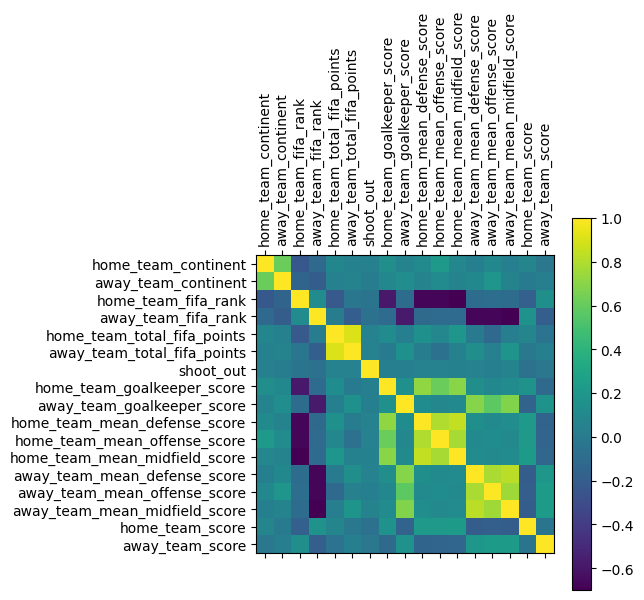
\includegraphics[width=\textwidth]{images/correlationMatrix.png}
    \caption{Matriz de correlaciones del conjunto de datos}
    \label{Conjunto-Datos-Matriz-Correlaciones}
\end{figure}

\begin{figure}[H]
    \centering
    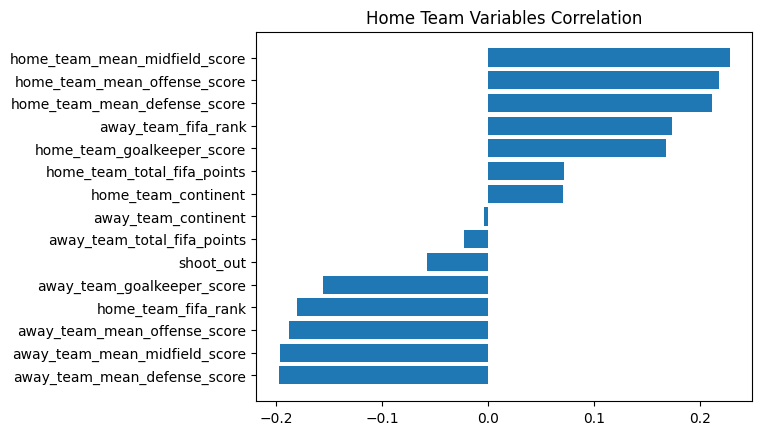
\includegraphics[width=\textwidth]{images/homeTeamCorrelation.png}
    \caption{Correlaciones de la variable home\_team\_score}
    \label{Conjunto-Datos-Home-Correlaciones}
\end{figure}

\begin{figure}[H]
    \centering
    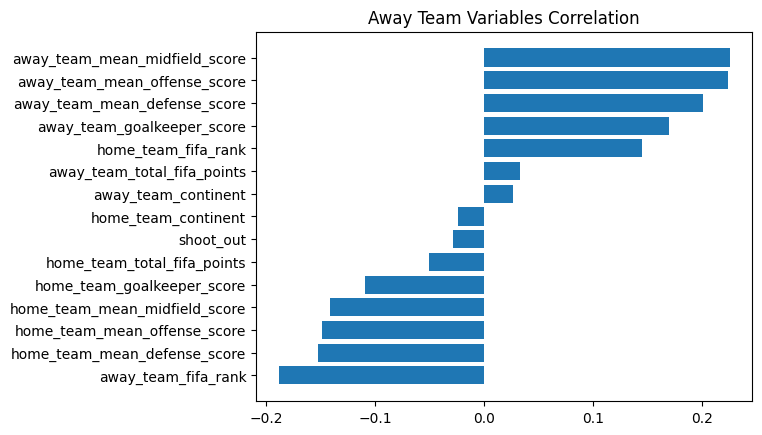
\includegraphics[width=\textwidth]{images/awayTeamCorrelation.png}
    \caption{Correlaciones de la variable away\_team\_score}
    \label{Conjunto-Datos-Away-Correlaciones}
\end{figure}

\newpage